\subsubsection{Fixing $a_L = a_R = b_L = b_R = 1$}

If you compare the functions in the cobwebs \Crefrange{fig:quad.full.CobwebA}{fig:quad.full.CobwebB} to the functions of the original model in \Crefrange{fig:yunus.2pi.CobwebA2}{fig:yunus.2pi.CobwebD2} you can see some differences.
One is, that the right end of the branches $\B$ and $\D$ is higher than the left part.
To get our model to look a little more like the original model, we now skew the branches by fixing also $b_L = b_R = 1$

The 2D scan for the periods when varying $c_L$ and $c_R$ now looks different.
\Cref{fig:quadratic.full.skew.2d.full} shows the full scan, while \Cref{fig:quadratic.full.skew.2d.z1} shows an enhanced version of it, depicting the artefact in the middle of the left half of the full scan.
\Cref{fig:quadratic.full.skew.2d.c} shows an enhanced version of the 2D scans depicting an interesting area where some cobwebs were taken.
The area is where a wing with stable cycles of period 12 connects with a wing of the same period.
There is a red line in the figure, it marks where the cobwebs are taken.

\begin{figure}
    \centering
    \begin{subfigure}{0.4\textwidth}
        \centering
        \includegraphics[width=\textwidth]{21_Quadratic_mod6/Skew/2D_Period_SFull/result.png}
        \caption{Full}
        \label{fig:quadratic.full.skew.2d.full}
    \end{subfigure}
    \begin{subfigure}{0.4\textwidth}
        \centering
        \includegraphics[width=\textwidth]{21_Quadratic_mod6/Skew/2D_Period_SZoomed1/result.png}
        \caption{Zoomed}
        \label{fig:quadratic.full.skew.2d.z1}
    \end{subfigure}
    \caption{2D Scan of Full Skewed Quadratic Model}
\end{figure}

\begin{figure}
    \centering
    \includegraphics[width=0.4\textwidth]{21_Quadratic_mod6/Skew/2D_Period_SC/result.png}
    \caption{2D Scan of Interesting Area of Full Skeqed Quadratic Model}
    \label{fig:quadratic.full.skew.2d.c}
\end{figure}

\Cref{fig:quad.full.skew.c.Cobwebs} shows all the cobwebs taken along the red line in \Cref{fig:quadratic.full.skew.2d.c}.
The first one, \Cref{fig:quad.full.skew.c.CobwebA}, shows a cycle with period 12.
Its symbolic sequence is $\A^4\B^2\C^4\D^2$.
The last cobweb, \Cref{fig:quad.full.skew.c.CobwebC}, also shows a 12-cycle, this time with symbolic sequence $\A^3\B^3\C^3\D^3$.
Here, one point from branches $\A$ and $\C$ moved to branches $\B$ and $\D$, the same thing that happened in the original model.
And in the middle, there is also coexistence of two 12-cycles.
This is depicted in \Cref{fig:quad.full.skew.c.CobwebB}.
The difference is, that in this case, the symbolic sequences of the two coexisting 12-cycles are $\A^4\B^2\C^4\D^4$ and $\A^3\B^3\C^3\D^3$.
This is different from the original model because there the symbolic sequences were $\A^3\B^3\C^2\D^4$ and $\A^2\B^4\C^3\D^3$, which were different from both 12-cycles existing outside the area of coexistence.
Here, the 12-cycles existing outside the coexistence area continue to exist inside it.

\begin{figure}
    \centering
    \begin{subfigure}{0.3\textwidth}
        \centering
        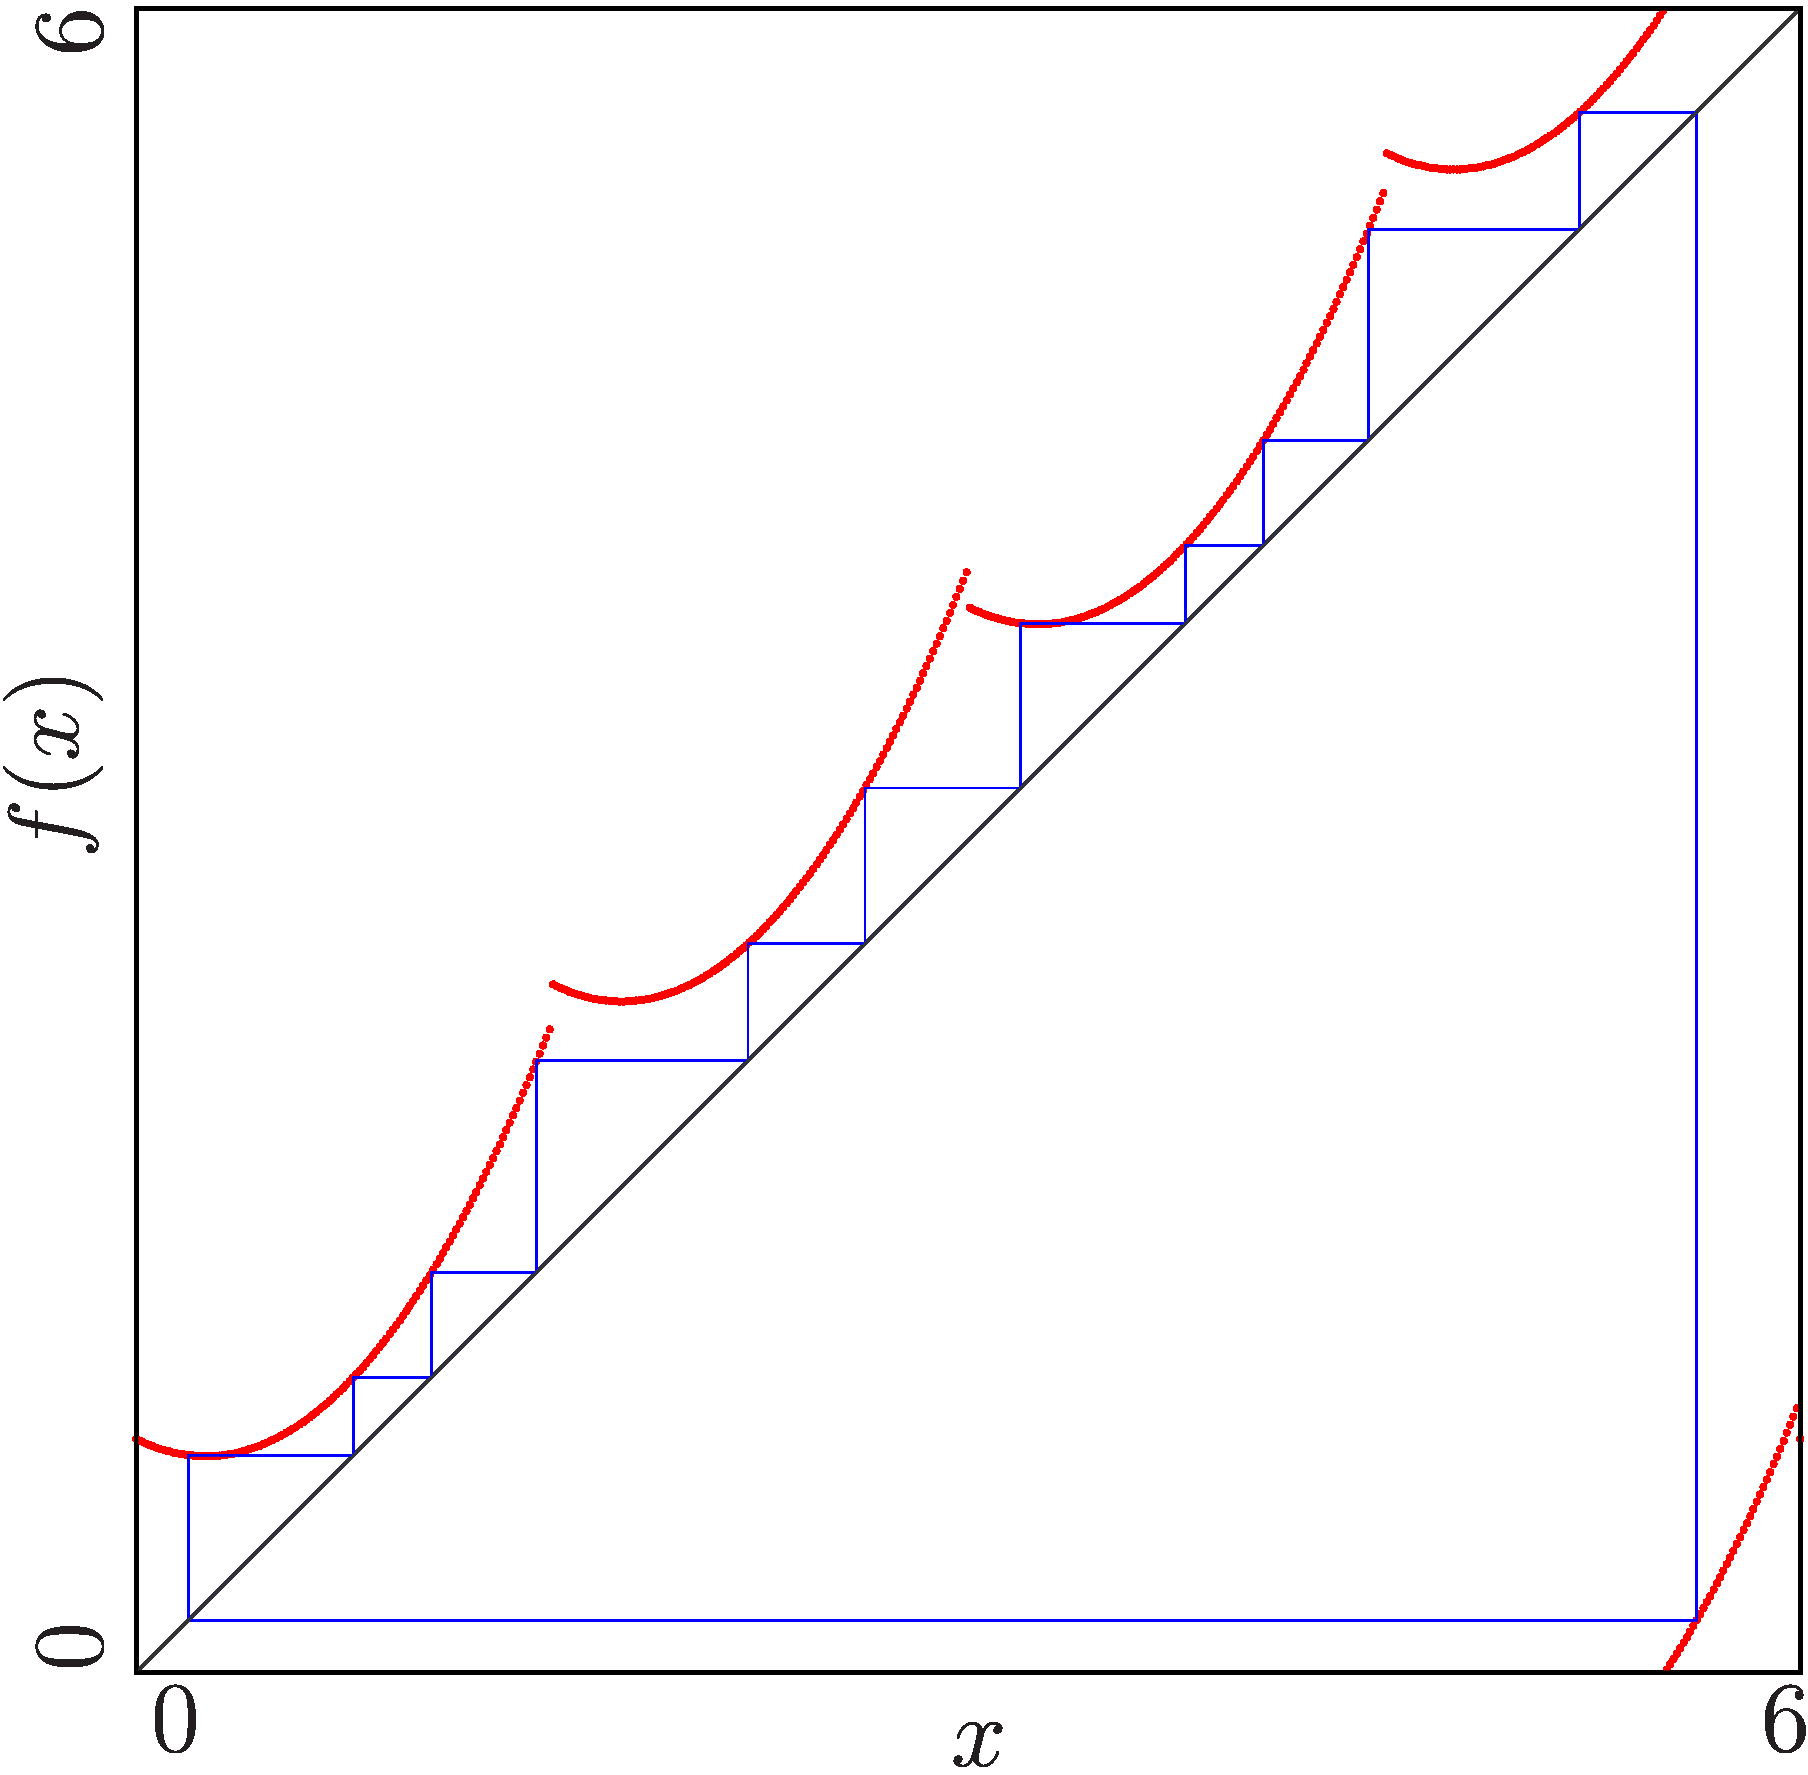
\includegraphics[width=\textwidth]{21_Quadratic_mod6/Skew/Cobweb_SC/result_A.png}
        \caption{Before border}
        \label{fig:quad.full.skew.c.CobwebA}
    \end{subfigure}
    \begin{subfigure}{0.3\textwidth}
        \centering
        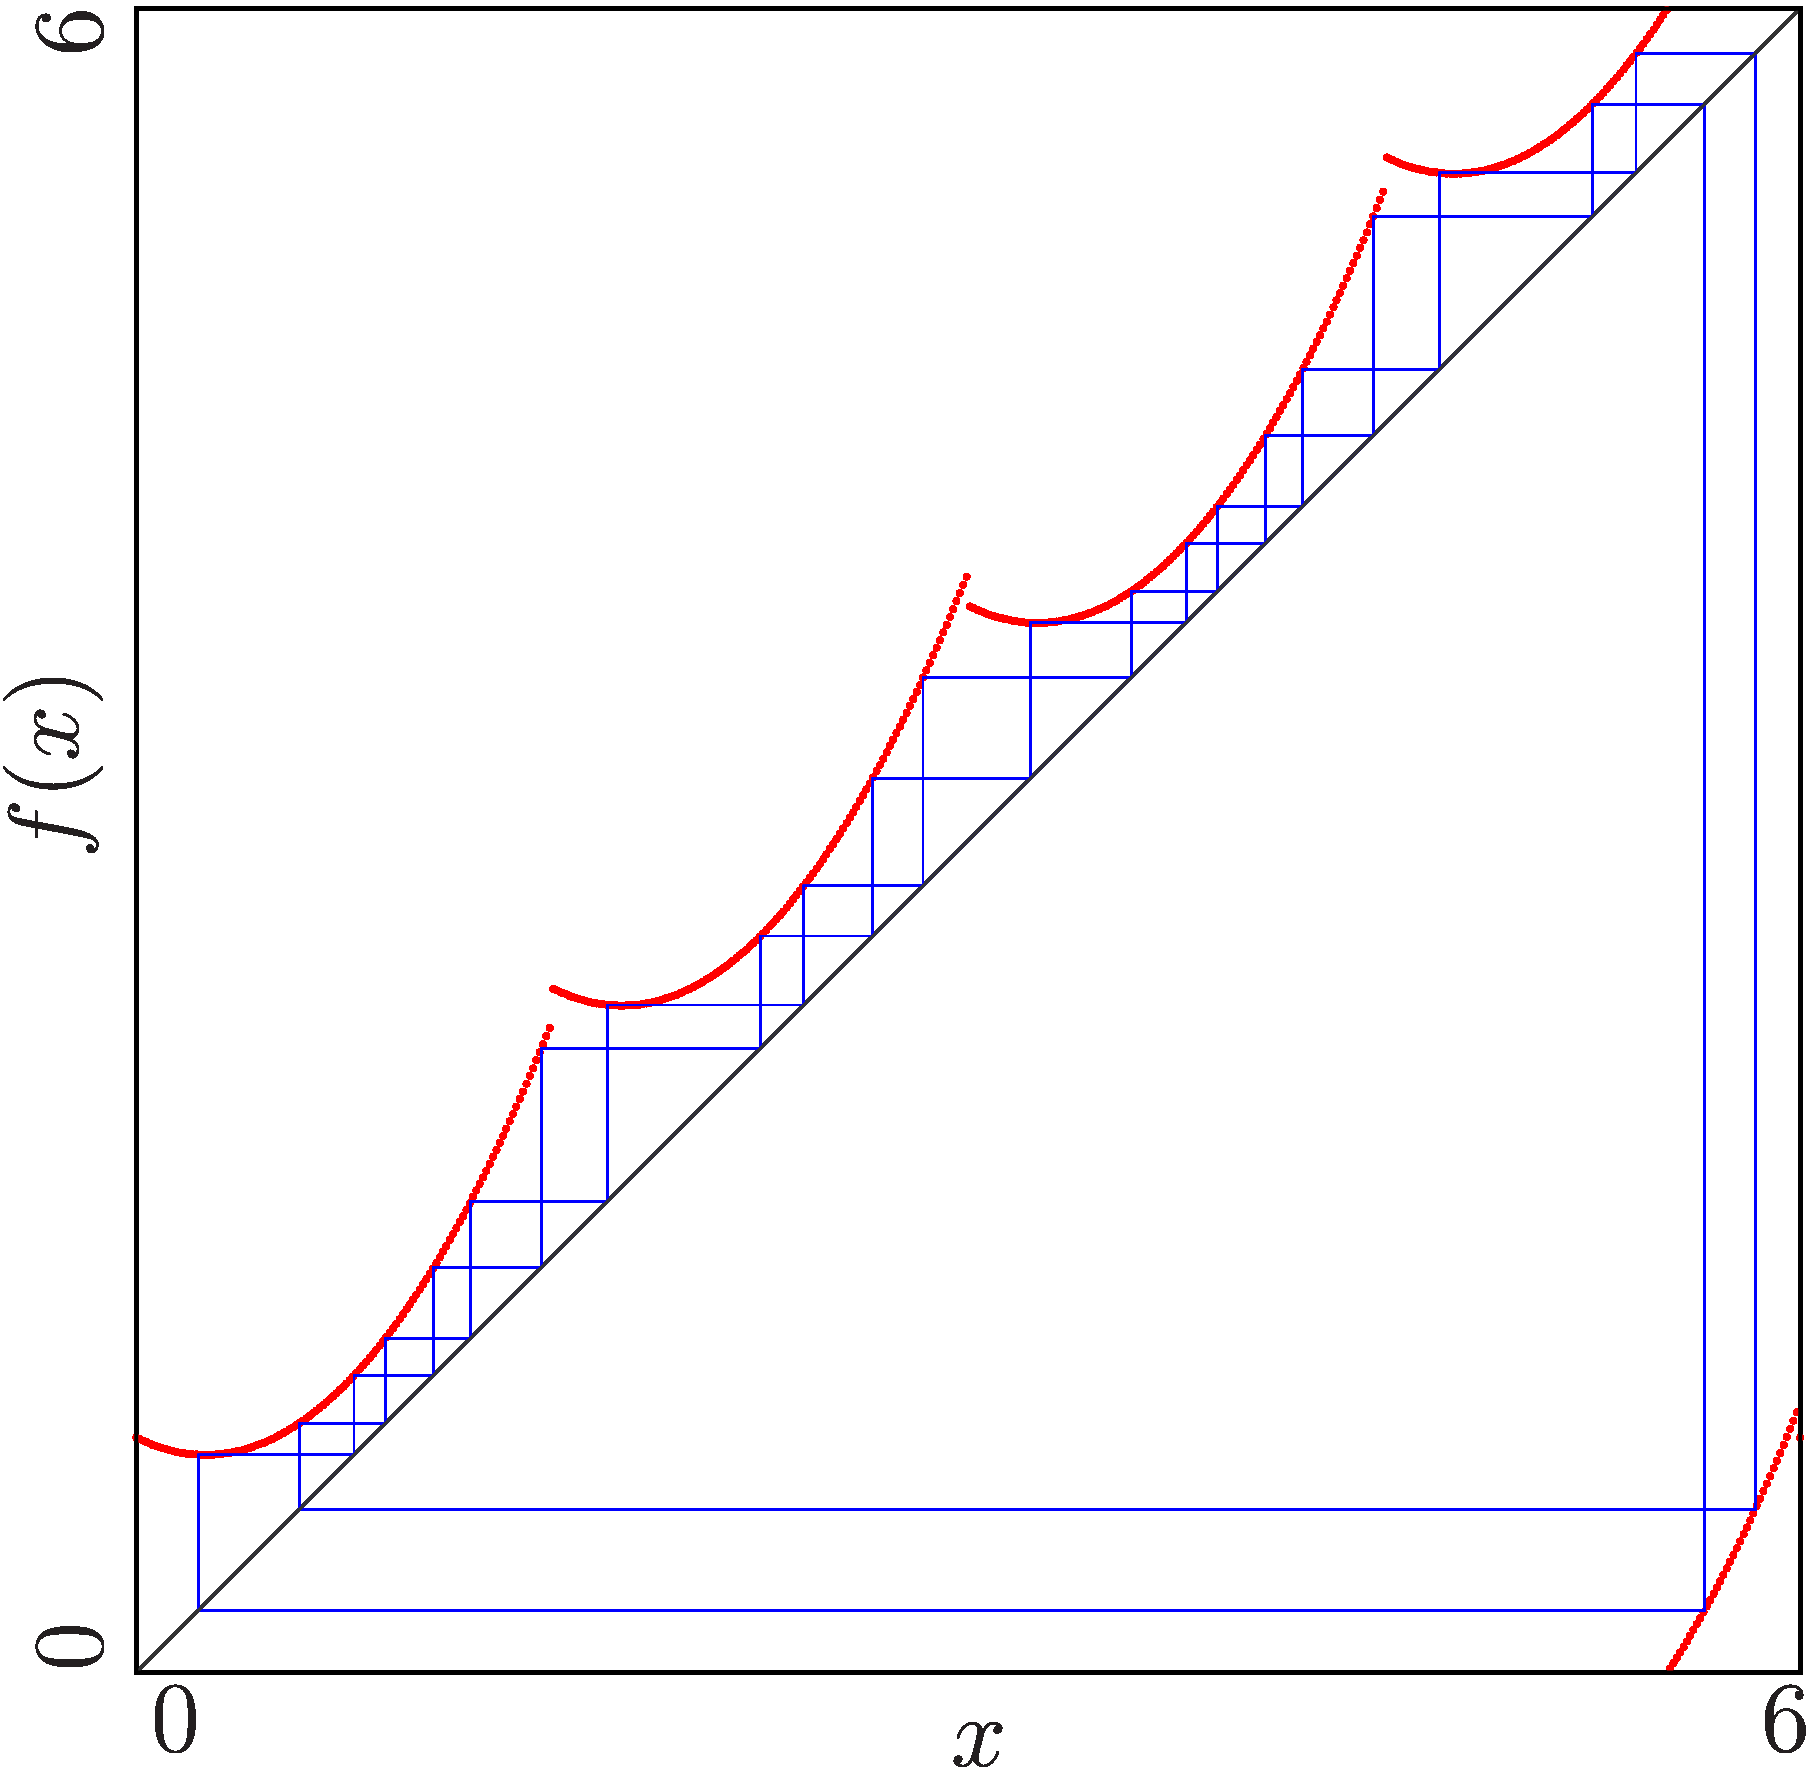
\includegraphics[width=\textwidth]{21_Quadratic_mod6/Skew/Cobweb_SC/result_B.png}
        \caption{At border}
        \label{fig:quad.full.skew.c.CobwebB}
    \end{subfigure}
    \begin{subfigure}{0.3\textwidth}
        \centering
        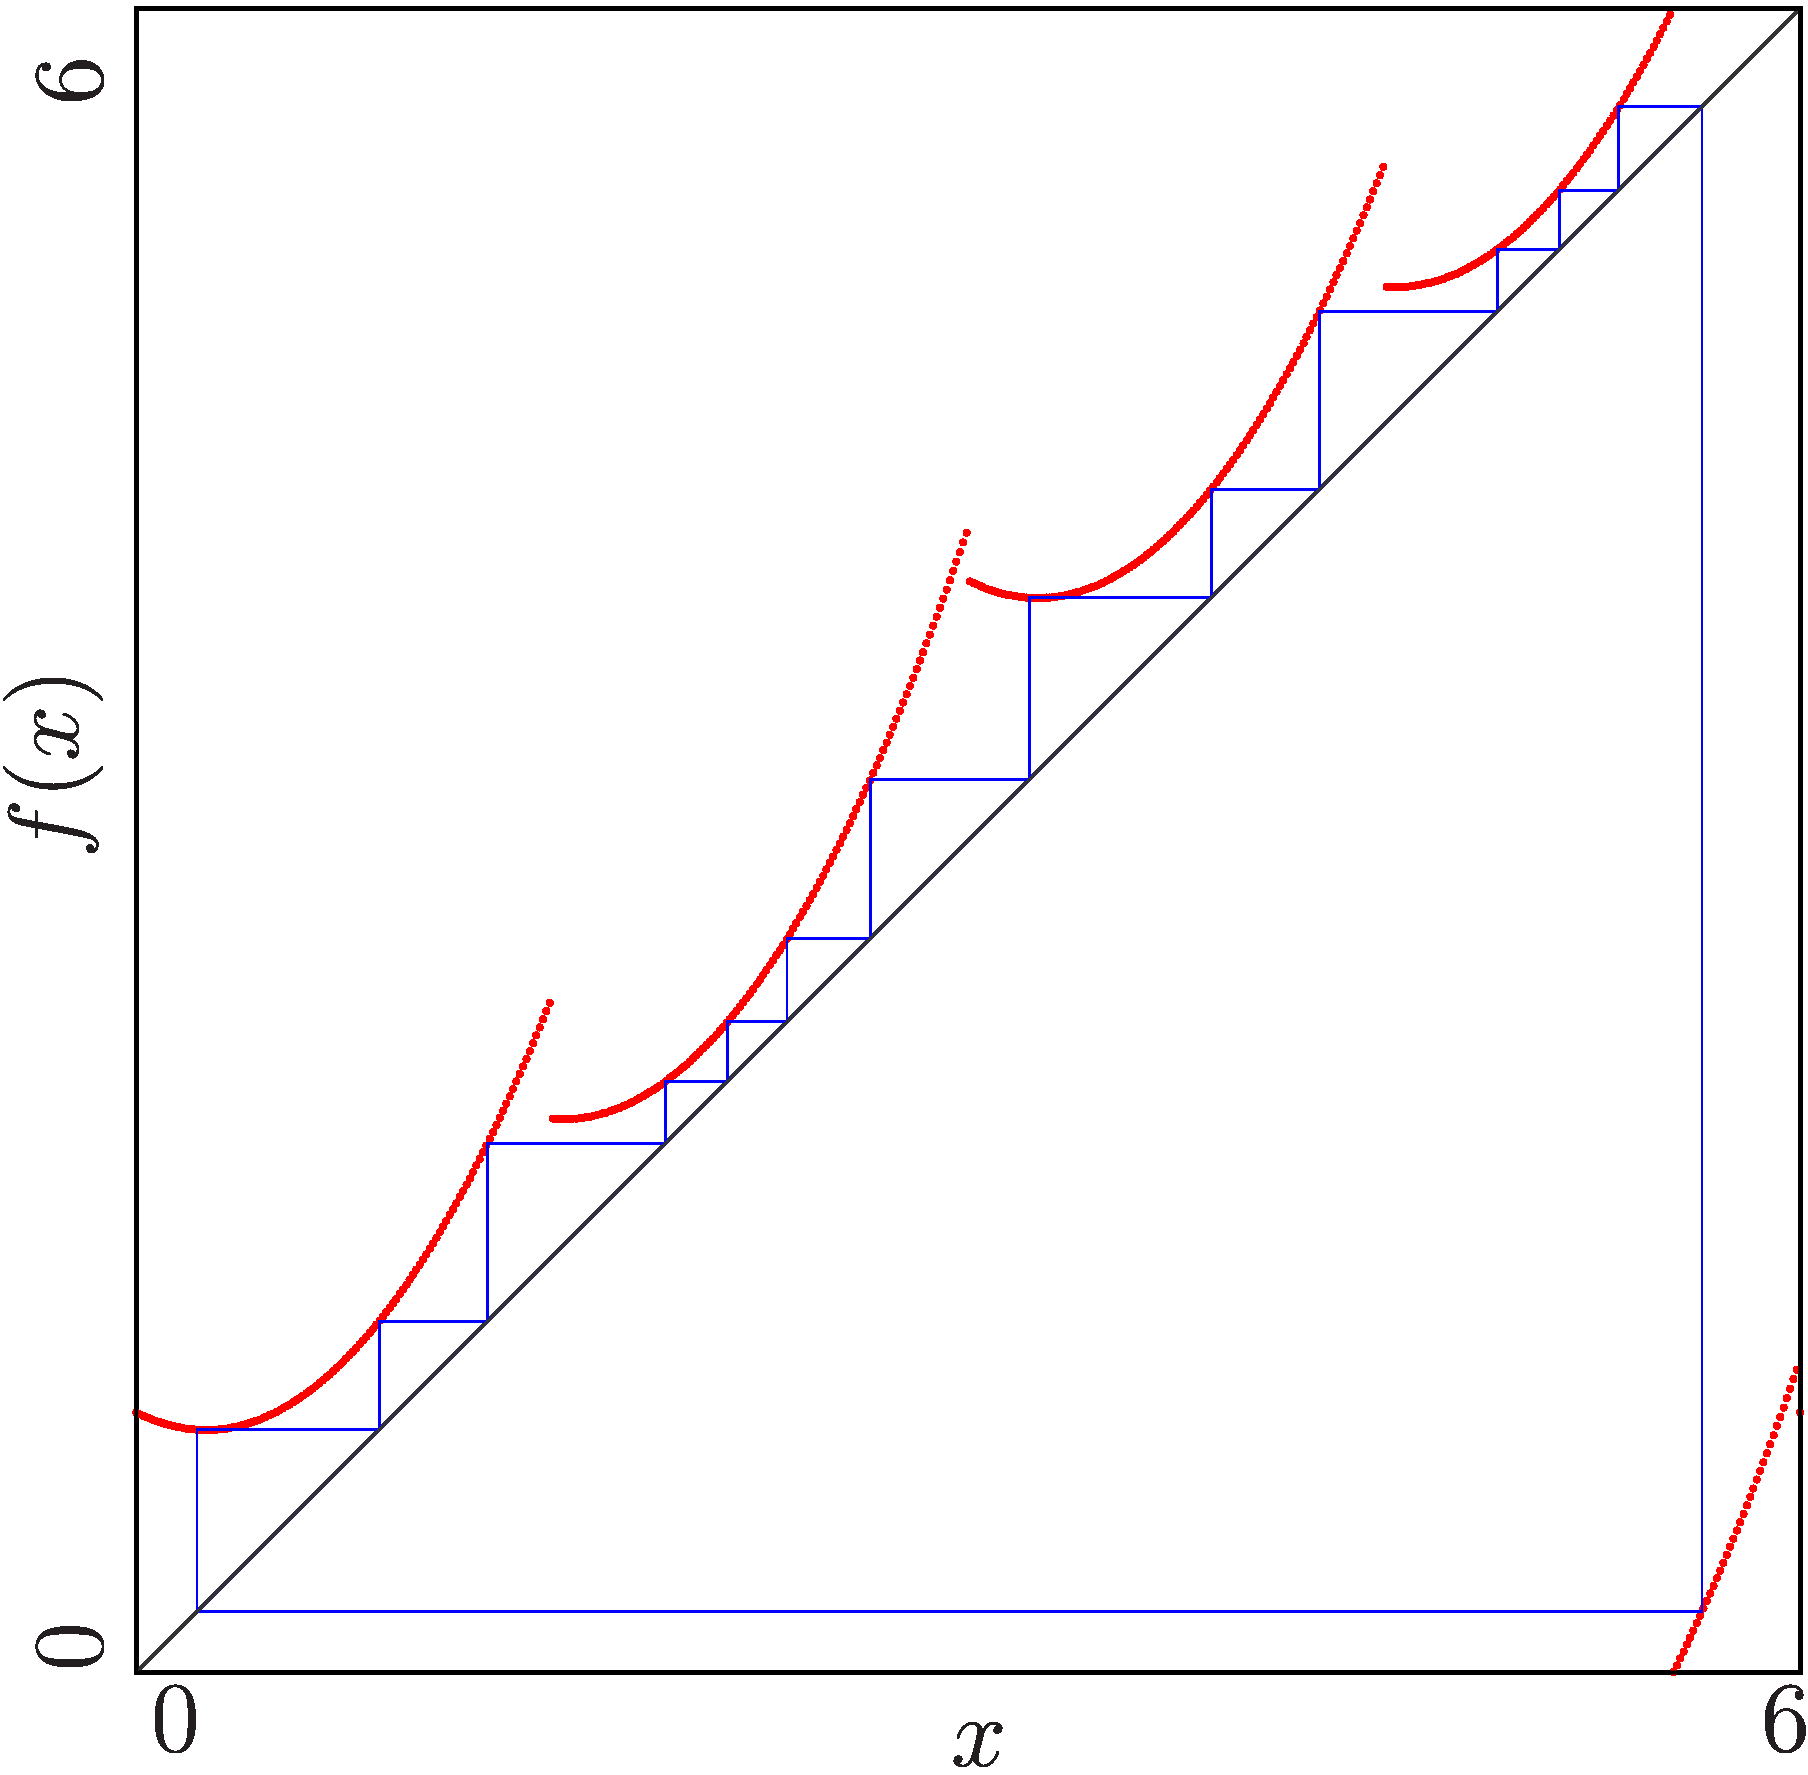
\includegraphics[width=\textwidth]{21_Quadratic_mod6/Skew/Cobweb_SC/result_C.png}
        \caption{After border}
        \label{fig:quad.full.skew.c.CobwebC}
    \end{subfigure}
    \caption{Cobwebs along marked line}
    \label{fig:quad.full.skew.c.Cobwebs}
\end{figure}
